\documentclass[a4paper]{article}

% (fold)
\usepackage{booktabs,amsmath,multirow} 
\usepackage{mathtools} % needed for next line
\mathtoolsset{showonlyrefs} 
\usepackage{fullpage}
\usepackage{calc}
\newcommand{\explain}[2]{\underbrace{#1}_{\parbox{\widthof{#1}}{\footnotesize\raggedright #2}}}

% only shows number of referenced equations
% \newcommand{\dpder}[3][]{\dfrac{\partial^{#1}#2}{\partial #3}} \addtolength{\oddsidemargin}{-.875in} \addtolength{\evensidemargin}{-.875in} \addtolength{\textwidth}{1.75in}
% \addtolength{\topmargin}{-.875in} \addtolength{\textheight}{1.75in}

% need for subequations
\usepackage{graphicx} 

% need for figures
\usepackage{verbatim}

% useful for program l,istings
\usepackage{color} 

% use if color is used in text
\usepackage{subfigure}

% use for side-by-side figures
\usepackage[pdfpagemode={UseOutlines},bookmarks=true,bookmarksopen=true, bookmarksopenlevel=0,bookmarksnumbered=true,hypertexnames=false, colorlinks,linkcolor={blue},citecolor={blue},urlcolor={red}, pdfstartview={FitV},unicode,breaklinks=true]{hyperref} 

% use for hypertext links, including those to external documents and URLs
\newcommand{\ajp}{AJP} 
\newcommand{\ig}{ 
\includegraphics} 
\newcommand{\tu}{\textup} \hypersetup{urlcolor=blue, colorlinks=true} 

% Colors hyperlinks in blue - change to black if annoying
% don't need the following. simply use defaults
\setlength{\baselineskip}{16.0pt} 

% 16 pt usual spacing between lines
\begin{comment}
	\pagestyle{empty} 
	
	% use if page numbers not wanted
\end{comment}

% Specifies the directory where pictures are stored
% above is the preamble (end)
\def\hpage{0.48\textwidth}
\def\MyWidth{0.71\textwidth} % textwidth for multiple graphs
\begin{document} 
\title{Homework 4, High-resolution shock-capturing methods} 
\author{Kevin Mead}

%\affiliation{KTH Royal Institute of Technology, Electrotechnical Modelling} \email{kmead@kth.se}
\date{\today} 
\maketitle 
\section{Shallow water with non-horizontal bottom} 

% (fold)
\label{sec:shallow_water_with_non_horizontal_bottom}

The shallow water model of HW2 is now extended to a non-horizontal bottom ``bathymetry'' ${B(x)}$. 
\begin{align}
	\begin{pmatrix}
		h_t\\
		hu_t 
	\end{pmatrix}
	+ 
	\begin{pmatrix}
		h_x u + h u_x\\h u u_x + gh( h_x + B_x ) 
	\end{pmatrix}
	= 
	\begin{pmatrix}
		0\\
		0 
	\end{pmatrix}
	\label{eq:originalEquation} 
\end{align}
\begin{description}
	\item[a)] Show that still water ($u=0$) must have, as it should, a horizontal water level. 
	
	If $u=0$ for all space and time, then $u_t$ and $u_x$ are also zero. Equation~\eqref{eq:originalEquation} becomes 
	\begin{equation}
		\begin{pmatrix}
			h_t\\0 
		\end{pmatrix}
		+ 
		\begin{pmatrix}
			0\\gh( h_x + B_x ) 
		\end{pmatrix}
		= 
		\begin{pmatrix}
			0\\0 
		\end{pmatrix}
		\label{eq:equationIfUiszero} 
	\end{equation}
	This means that $h_t=0$ and $h_x=-B_x$. We know that $B(x)_t=0$ because it isn't a function of time. The total height, $D(x,t)$, is $D(x,t) = h(x,t) + B(x)$. A horizontal water level means that $D(x,t) = \text{constant}$ and $D(x,t)_x=D(x,t)_t=0$. Equation~\eqref{eq:proveHorizontalWaterlevel} shows that derivatives with respect to $x$ and $t$ are zero and therefore showing that the total height $D(x,t)$ is constant. 
	\begin{align}
		D(x,t)_x &= h_x + B_x = h_x + (-h_x) = 0\\
		D(x,t)_t &= h_t + B_t = 0 + 0 = 0 \label{eq:proveHorizontalWaterlevel} 
	\end{align}
	
	\item[b)] Write the equation in conservation form for $h$ and $m=hu$. 
	\begin{equation}
		\begin{pmatrix}
			h\\m 
		\end{pmatrix}
		_t + 
		\begin{pmatrix}
			m\\f_2(h,m) 
		\end{pmatrix}
		_x = 
		\begin{pmatrix}
			0\\s(h,m,x) 
		\end{pmatrix}
		\label{eq:proveThisEquation} 
	\end{equation} % (eq:proveThisEquation)
	The first equation in Equation~\eqref{eq:proveThisEquation} is proved using the product rule, $m_x = h_x u + h u_x$. The second equation needs to be written out explicitly and solved for the unknowns. Substituting $m_t = h_t u + h u_t$ into Equation~\eqref{eq:proveThisEquation} 
	\begin{align}
		(h_t u + h u_t) + [h u u_x + gh( h_x + B_x )] = h_t u  \label{eq:firstToConservation} 
	\end{align}
	
	% (eq:firsttoconservation)
	and substituting $u=m/h$ and $h_t=-m_x$ 
	\begin{equation}
		m_t + [h \left(\frac{m}{h}\right) \left(\frac{m}{h}\right)_x + gh( h_x + B_x )] = (-m_x) \left(\frac{m}{h}\right) \label{eq:secondtoConservation} 
	\end{equation}
	
	% (eq:secondtoconservation)
	and bringing x and t derivatives together and putting derivatives other than $h$ or $m$ to the source function 
	\begin{align}
		m_t + [\underbrace{m \left(\frac{m}{h}\right)_x + m_x \left(\frac{m}{h}\right)}_{(m^2/h)_x} + \underbrace{gh h_x}_{(gh^2/2)_x}] &= -gh B_x \label{eq:thirdConservation} \\
			m_t + (\underbrace{\frac{m^2}{h} + \frac{gh^2}{2}}_{f_2(h,m)})_x &= \underbrace{-gh B_x}_{s(h,m,x)}\label{eq:fourthConservation}
	\end{align} % (eq:thirdconservation)
	Equation~\eqref{eq:proveThisEquation} written in conservation form becomes,
\begin{equation}
	\begin{pmatrix}
		h\\m 
	\end{pmatrix}
	_t + 
	\begin{pmatrix}
		m\\\frac{m^2}{h} + \frac{gh^2}{2} 
	\end{pmatrix}
	_x = 
	\begin{pmatrix}
		0\\ -g h B_x
	\end{pmatrix}
	\label{eq:proveThisEquationSolved}
\end{equation} % (eq:provethisequationsolved)
\end{description}

% section shallow_water_with_non_horizontal_bottom (end)



%!TEX root = /Users/kevin/SkyDrive/KTH Work/LaTeX Reports/HW4-High Resolution shock-capturing methods/HW4_High_Resolution_shock_capturing_methods.tex
\section{First order Roe scheme} 
\subsection{Roe tests with flat bottom} % (fold)
\label{sub:roe_tests_with_flat_bottom}

% subsection roe_tests_with_flat_bottom (end)
% (fold)
\label{sec:first_order_roe_scheme} 
\begin{enumerate}
	\item 
	\begin{enumerate}
		\item Explain how to choose m(x,0), to make a single pulse (not two!) based on the linearized problem. 
		
		You can make it a single pulse by giving the wave an initial speed proportional to its height in one direction. Since $m=hv$, we can set m to $hc$, where the characteristic speed is $c=\sqrt{gH}$, and $H=0$ since we want a linearized approximation.
		
		\item Use this initial data and run the Roe solver with n=80, 160, 320 and the CFL number as large as possible without instability, until the wave has been fully reflected at L. Plot the wave shapes. 
		
		Figure~\ref{fig:Figure21} shows the plots using different N values.  The N value seemed to affect the sharpness of the front edge of the wave. As N increased, the sharpness increased.  
		\begin{figure}
			[htbp] \centering 
			\subfigure[$N=80$ \label{fig:Figures_plot2p1_n_is_80}]{ 
			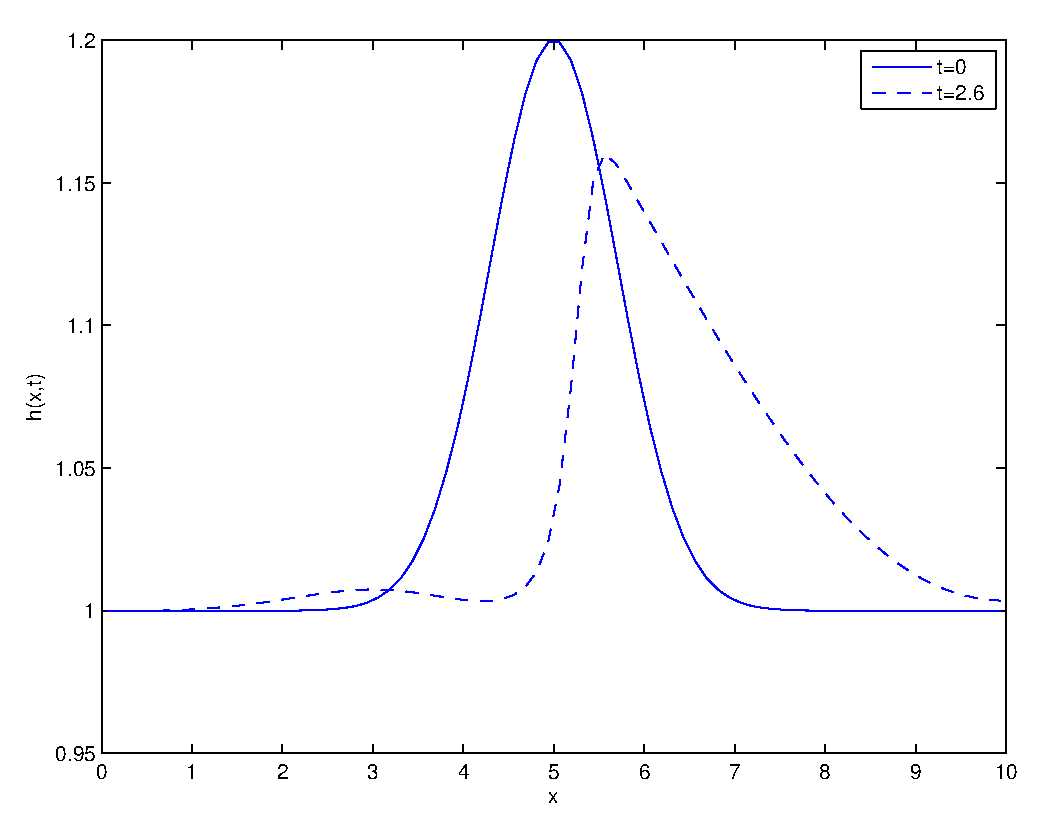
\includegraphics[width=\hpage]{Figures/plot2p1_n_is_80.eps}} \hspace{5pt} 
			\subfigure[$N=160$ \label{fig:Figures_plot2p1_n_is_80}]{ 
			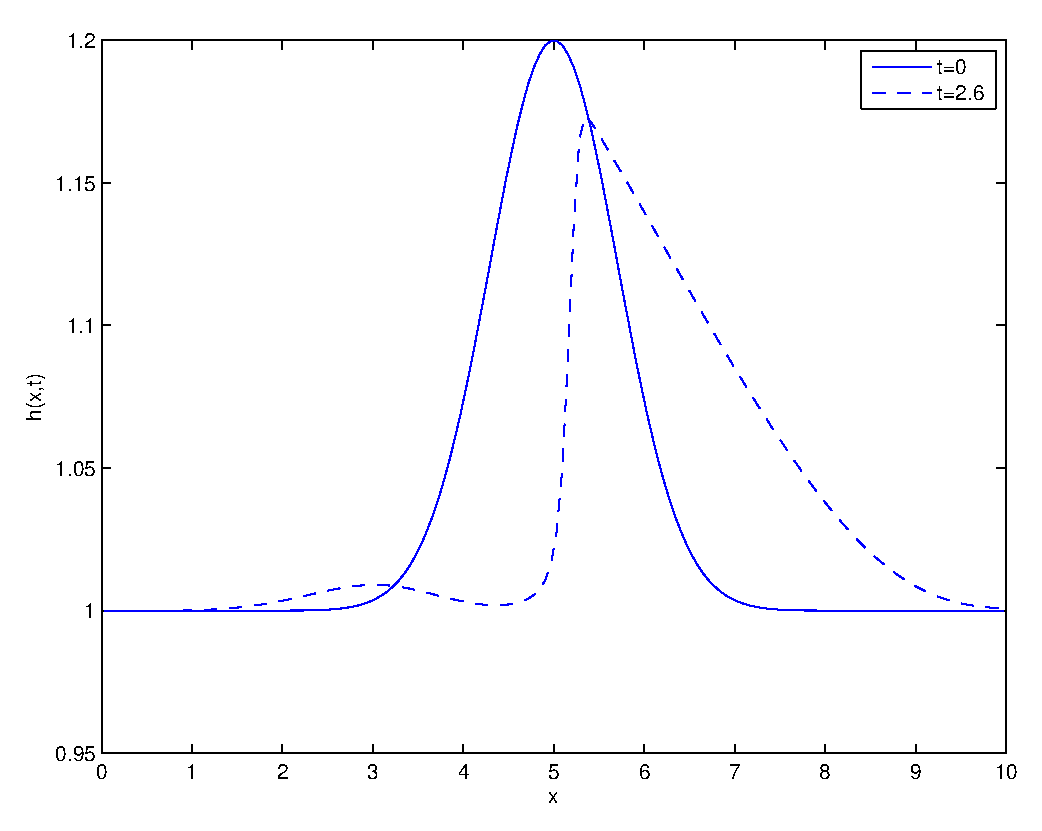
\includegraphics[width=\hpage]{Figures/plot2p1_n_is_160.eps}} \label{fig:Figures_plot2p1_n_is_160}
			\subfigure[$N=320$ \label{fig:Figures_plot2p1_n_is_320}]{
			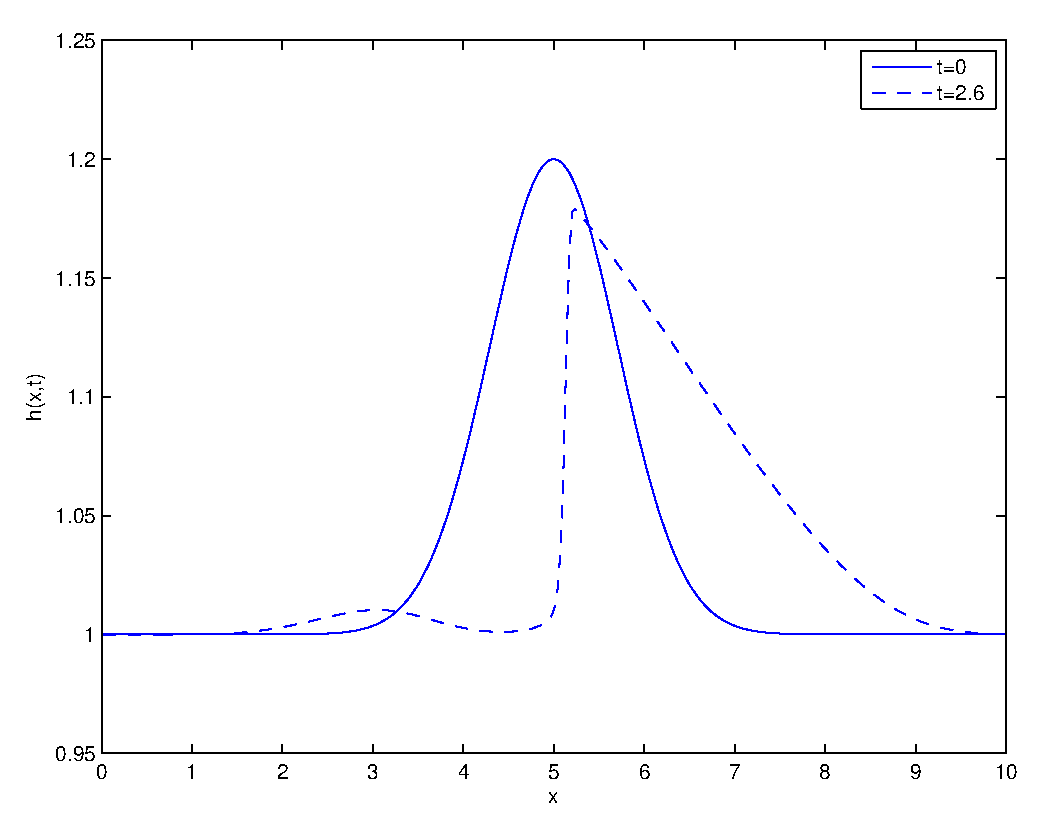
\includegraphics[width=\hpage]{Figures/plot2p1_n_is_320.eps}}
			\caption{These are the plots with different N values.  The CFL condition was set to 80\% of the value that would be ideal for a linear problem. The wave edges get sharper when $N$ is increased} 
			\label{fig:Figure21}
		\end{figure}
		
		\item Compare with solutions obtained using your Lax-Friedrichs solver from HW2. 
		
		The solution obtained here looks very similar to the Lax-Friedrichs solver from HW2 as the shape of the wave forms a sharp edge and looks like a triangle instead of a Gaussian.  This solution isn't stable at the CFL condition and we must make the time step a little smaller.  The Lax-Friedrich solution was also not stable at the CFL condition, but I was forced to decrease the time step by a much larger amount in order to see stability for a few seconds.
		\item Comment about order of accuracy, dissipation and dispersion. 
		The dissipation around the edges decreases as we increase the value of N.  But increasing the value of N too much will only cause instabilities.
		
		\item Then try also a higher pulse, say a = 2H. Comment on how well the single pulse initial data works. 
		
		A pulse with $a>1/5 H$ gives unstable results using a time step of 80\% of the CFL condition, so I had to reduce it to 40\% in order to get the results shown in Figure~\ref{fig:Figure21d}.  This figure is different from Figure~\ref{fig:Figure21} in that the height of the left moving pulse isn't as negligible as it once was.  The overlap of the smaller wave is much more noticeable when $a$ is large compared to H. 
		
		\begin{figure}
			[htbp] \centering 
			\subfigure[$N=80$ \label{fig:Figures_plot2p1_n_is_80_a_2}]{ 
			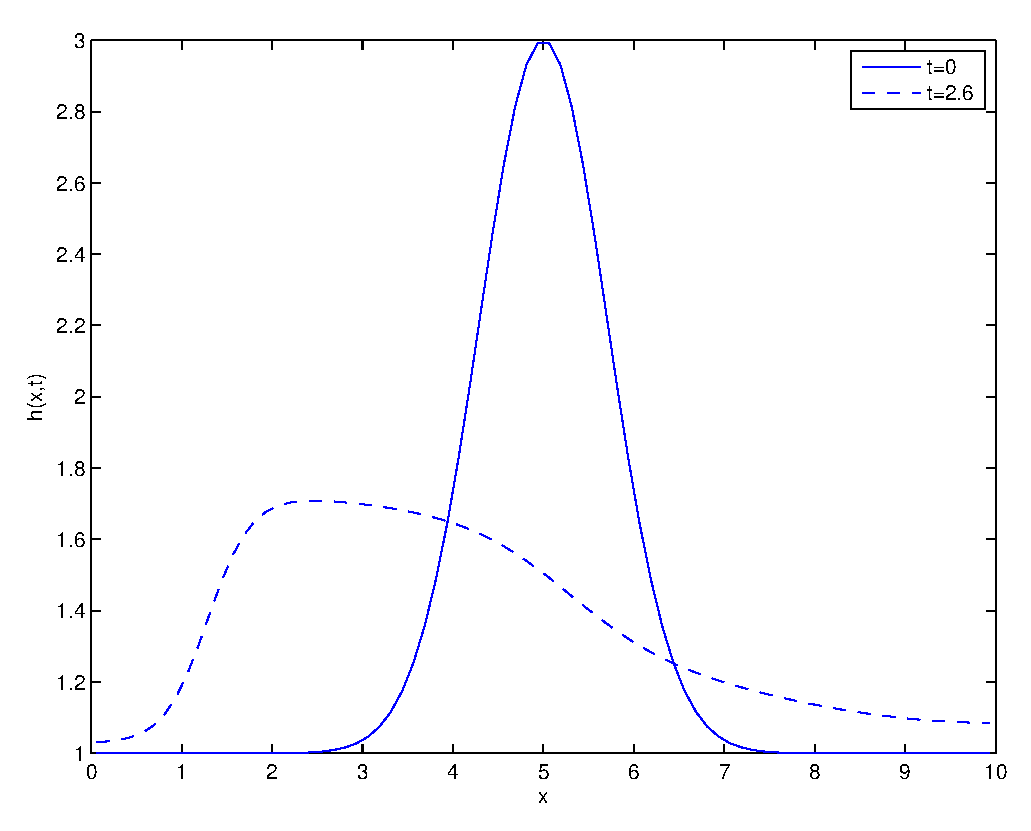
\includegraphics[width=\hpage]{Figures/plot2p1_n_is_80_a_2.eps}} \hspace{5pt} 
			\subfigure[$N=160$ \label{fig:Figures_plot2p1_n_is_80_a_2}]{ 
			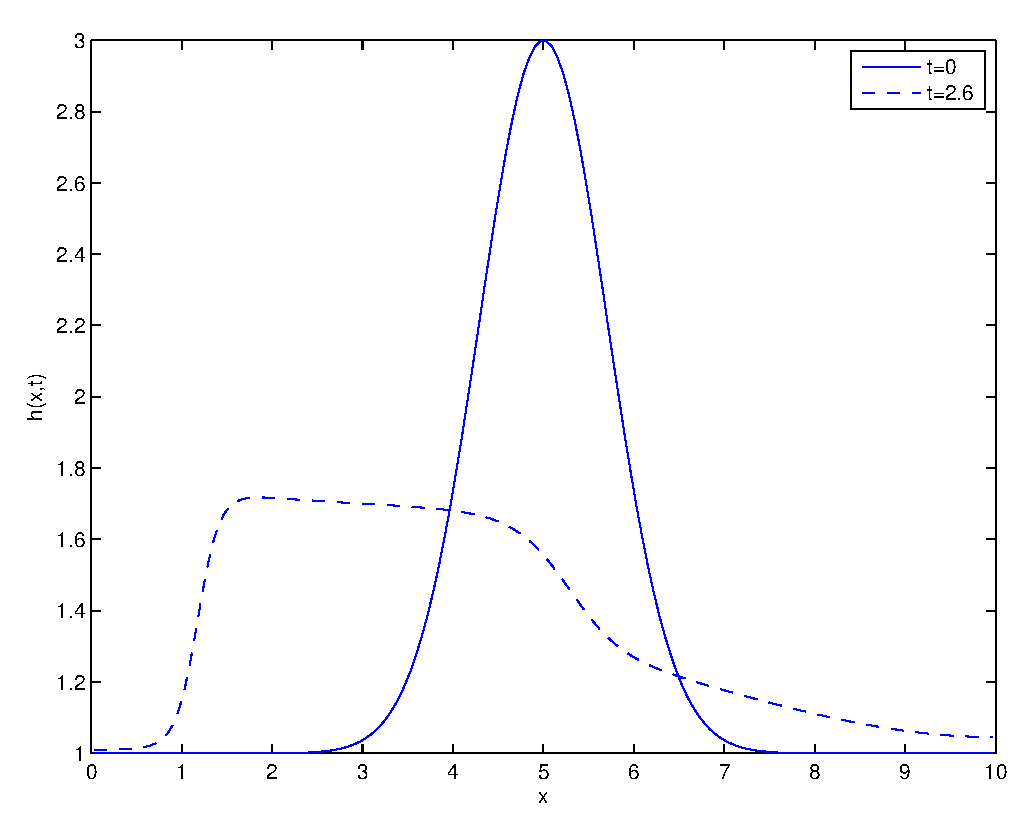
\includegraphics[width=\hpage]{Figures/plot2p1_n_is_160_a_2.eps}} \label{fig:Figures_plot2p1_n_is_160_a_2}
			\subfigure[$N=320$ \label{fig:Figures_plot2p1_n_is_320_a_2}]{
			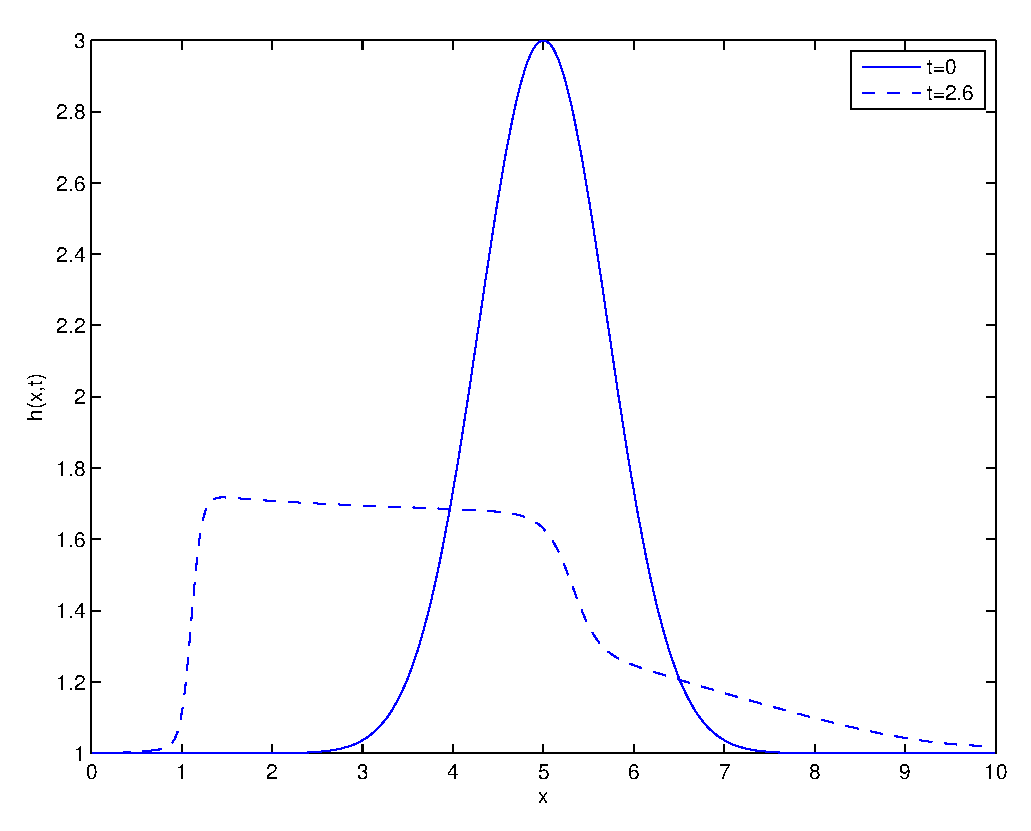
\includegraphics[width=\hpage]{Figures/plot2p1_n_is_320_a_2.eps}}
			\caption{These are the plots with different N values.  The CFL condition was set to 40\% of the value that would be ideal for a linear problem. The wave edges get sharper when $N$ is increased, but changing the value of $a$ has also changed the characteristic speed and shape of the wave after it recombines with its small wave that moves leftward.} 
			\label{fig:Figure21d}
		\end{figure}
		
	\end{enumerate}
\end{enumerate}

% section first_order_roe_scheme (end)

%!TEX root = /Users/kevin/SkyDrive/KTH Work/LaTeX Reports/HW4-High Resolution shock-capturing methods/HW4_High_Resolution_shock_capturing_methods.tex
\subsection{Steady solutions with non-horizontal bottom} % (fold)
\label{sub:steady_solutions_with_non_horizontal_bottom}


If the flow is sub-critical, $|u(x)|<\sqrt{gh(x)}$, then for Dirichlet boundary conditions, we should set $h(x)$ to be large enough to satisfy the sub-critical condition at the boundaries.  The same should be done for super-critical conditions at the boundaries.




% subsection steady_solutions_with_non_horizontal_bottom (end)


%!TEX root = /Users/kevin/SkyDrive/KTH Work/Period 3 2014/DN2255/Homework/4/HW4-High Resolution shock-capturing methods/HW4_High_Resolution_shock_capturing_methods.tex
\subsubsection{Smooth Steady state solutions} 

% (fold)
\label{subsub:smooth_steady_state_solutions}

% subsubsection smooth_steady_state_solutions (end)
Figure~\ref{fig:Figures_steadySolutionsp1_n_is_80_a_0} shows the plot with the source term.
% (eq:bxequation)
\begin{figure}
	[htbp] \centering 
	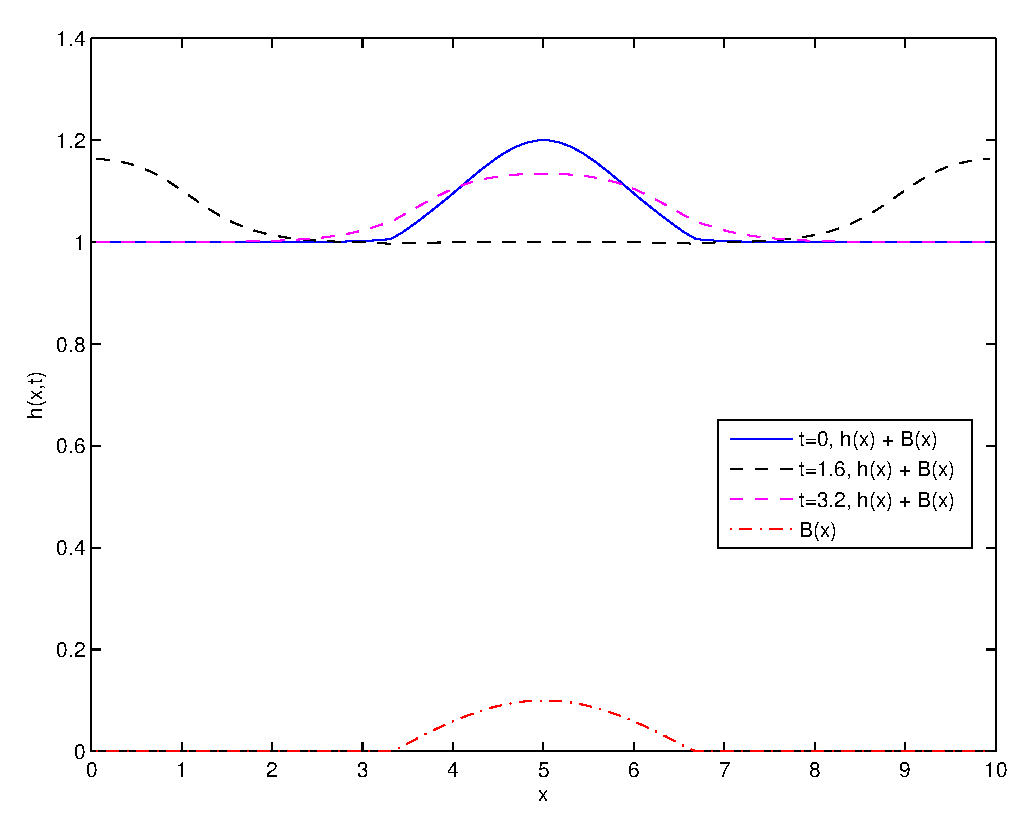
\includegraphics[width=\MyWidth]{Figures/steadySolutionsp1_n_is_80_a_0.eps} \caption{Solution with an uneven bottom that contributes to the wave shape and speed. The depth of the wave is is related to the bottom surface as well as its own surface.} \label{fig:Figures_steadySolutionsp1_n_is_80_a_0} 
\end{figure}

%(fig:Figures_steadySolutionsp1_n_is_80_a_0)
\begin{figure}
	[htbp] \centering 
	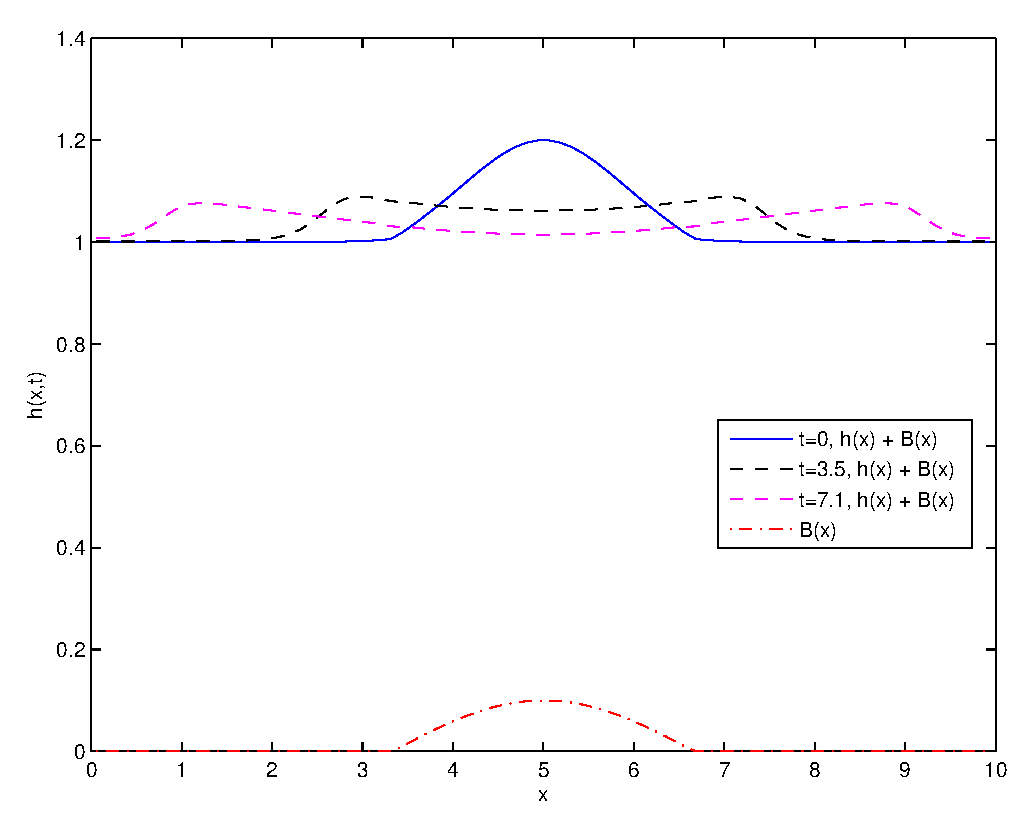
\includegraphics[width=\MyWidth]{Figures/critical_c2817_p1_n_is_80_a_0.eps} \caption{Subcritical condition} \label{fig:Figures_critical_c2817_p1_n_is_80_a_0} 
\end{figure}

%(fig:Figures_critical_c2817_p1_n_is_80_a_0)
\begin{figure}
	[htbp] \centering 
	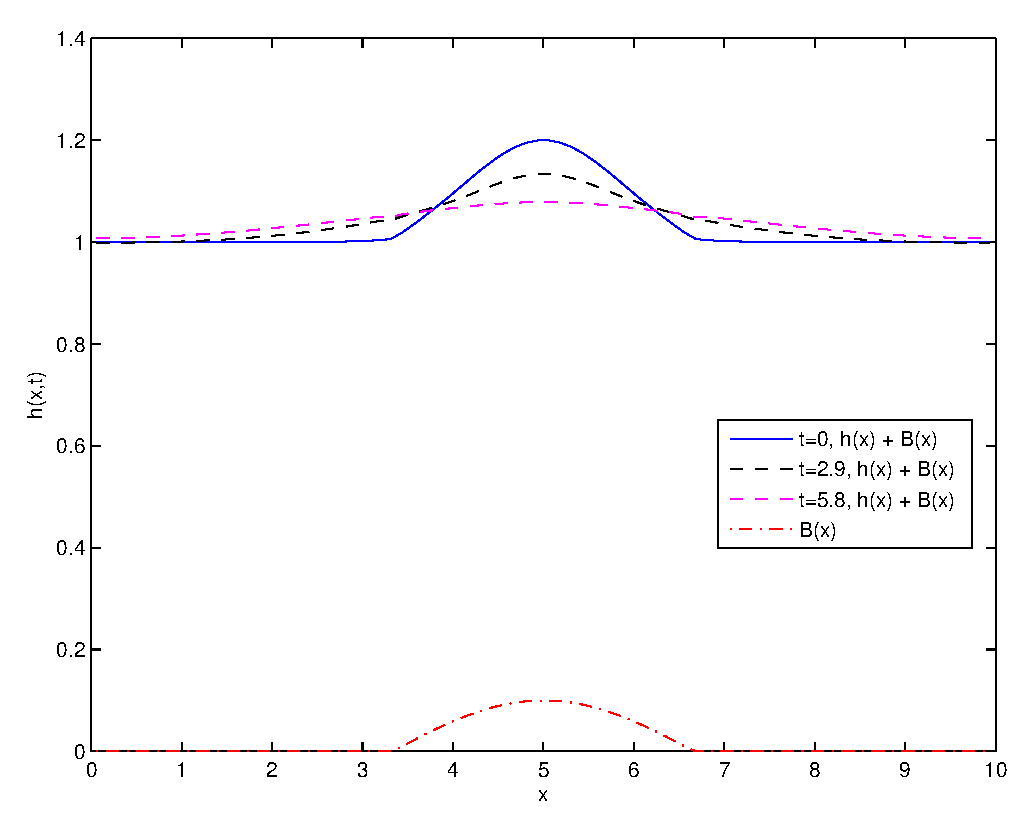
\includegraphics[width=\MyWidth]{Figures/critical_c3444_p1_n_is_80_a_0.eps} \caption{Super-critical} \label{fig:Figures_critical_c3444_p1_n_is_80_a_0} 
\end{figure}

%(fig:Figures_critical_c3444_p1_n_is_80_a_0)

\bibliographystyle{IEEEtran}
\bibliography{My_Book}
%\noindent Updated \today.} 
\end{document} 
